% PLEASE FILL IN THE PLACEHOLDERS <...>
%
% Diplomarbeit/Studienarbeit/IDP von <NAME>
% Diploma thesis of <NAME>
%
% Title: <TITLE>
%        <TITLE>
%
\documentclass[12pt,a4paper]{report}

%%%%%%%%%%%%%%%%%%%%%%%%%%%%%%%%%%%%%%%%%%%%%%%%%%%%%%%%%%%%

% PACKAGES:

% Define typearea
% a) Use automatic:
\usepackage[BCOR1cm]{typearea}
% b) Or use fixed: 
%\usepackage{geometry}
%\geometry{left=1.5cm,textwidth=18.5cm,top=1.5cm,textheight=26.5cm}

% Use German :
\usepackage[USenglish]{babel}
% Use list of tabels, etc. in table of contents:
\usepackage{tocbibind}
% German paragraph skip
\usepackage{parskip}
\usepackage{enumitem}
% Encoder:????
%\usepackage[utf-8]{inputenc}
\usepackage[utf8]{inputenc}
% Use A4-paper efficiently:
\usepackage{a4wide}
% Index-generation
\usepackage{makeidx}
% Einbinden von URLs:
\usepackage{url}
% Include .eps-files (needed also for the LKN-logo):
%\usepackage{epsf}
\usepackage{epsfig}
\usepackage{epstopdf}
% Special \LaTex symbols (e.g. \BibTeX):
\usepackage{doc}
% Include Graphic-files:
%\usepackage{graphics}
% Include Graphic-files:
\usepackage{graphicx}
% Include doc++ generated tex-files:
%\usepackage{docxx}
% Include PDF links
%\usepackage[pdftex, bookmarks=true]{hyperref}

\usepackage{amsmath}

%%%%%%%%%%%%%%%%%%%%%%%%%%%%%%%%%%%%%%%%%%%%%%%%%%%%%%%%%%%%

% OTHER SETTINGS:

% Pagestyle:
\pagestyle{headings}

% Avoid 'overhang':
\sloppy

% Choose language
\newcommand{\setlang}[1]{\selectlanguage{#1}\nonfrenchspacing}

%%%%%%%%%%%%%%%%%%%%%%%%%%%%%%%%%%%%%%%%%%%%%%%%%%%%%%%%%%%%

% TITLE:

\begin{document}

\thispagestyle{empty}
\newpage

\vspace{5cm}
\begin{center}
    \epsfxsize=4cm
    \epsfbox{LKN_Logo_klein.eps}
\end{center}

\parbox{15cm}{\begin{center} {\sf\bf 
                               \Large  Technische Universität München
                                \smallskip

                               \Large Lehrstuhl für Kommunikationsnetze
                               \smallskip
                              }

                              {\sf \large Prof. Dr.-Ing. Wolfgang Kellerer} 
              \end{center}}  %&

\vspace{4cm}

\begin{center}
        {\bf\Huge Master‘s Thesis} % Studienarbeit, Interdisziplinäres Projekt
\end{center}

\begin{center}
        \settowidth{\baselineskip}{0.4cm}
        {\LARGE 
        VM Selection Heuristic for Financial Exchanges on the Cloud
        }
\end{center}

\vfill         
{\settowidth{\baselineskip}{0.2cm}
\large\begin{tabular}[l]{ll}
Author: & Duclos-Cavalcanti, Daniel\\
Address: & 230 W 55th Street\\
         & 10019 New York, NY\\
         & U.S.A.\\
Matriculation Number: & 03692475\\
Supervisor: & Muhamadd Haseeb \& Navidreza Asadi\\
Begin: & 03. April 2024\\
End: & 03. October 2024
\end{tabular}}

%%%%%%%%%%%%%%%%%%%%%%%%%%%%%%%%%%%%%%%%%%%%%%%%%%%%%%%%%%%%

% MAIN PART:
% Independence and License statements
\thispagestyle{plain}


\vspace*{1cm}
With my signature below, I assert that the work in this thesis has been composed by myself independently and no source materials or aids other than those mentioned in the thesis have been used.



\vspace{2cm}

\hspace{1cm}\begin{tabular}{ccc}
\vspace{-0.3cm}München, 11.06.2014 	&\hspace{4cm} 		& \\
\rule{4.5cm}{0.4pt}					&					&\rule{4.5cm}{0.4pt}\\
Place, Date							&					& Signature			
\end{tabular}

           		






\vspace{4cm}
This work is licensed under the Creative Commons Attribution 3.0 Germany License. To view a copy of the license, visit http://creativecommons.org/licenses/by/3.0/de\\

Or\\

Send a letter to Creative Commons, 171 Second Street, Suite 300, San Francisco, California 94105, USA.

\vspace{2cm}



\hspace{1cm}\begin{tabular}{ccc}
\vspace{-0.3cm}München, 11.06.2014 	&\hspace{4cm} 		& \\
\rule{4.5cm}{0.4pt}					&					&\rule{4.5cm}{0.4pt}\\
Place, Date							&					& Signature	
\end{tabular}
% German abstract:
\setlang{german}
\thispagestyle{plain}

\section*{Kurzfassung} 
A short abstract of the thesis in German. 
% English abstract:
\setlang{USenglish}
\thispagestyle{plain}

\section*{Abstract}
A short abstract of the thesis in English. 



% Table of contents:
\tableofcontents  
% Introduction (Einleitung):
\chapter{Introduction}

This chapter should give a short overview over the whole thesis. It should provide background information on the thesis topic, introduce the task definition and give a short outlook on the rest of the thesis. 


% Text Body (Hauptteil)
% Could have multiple chaper-files, e.g.:
\chapter{Background}

% In this chapter, all background necessary to understand the thesis are introduced. The level of detail is such that 
% a colleague with similar background (no specialist!) is capable of understanding the contribution and impact of the thesis. 
% A discussion of state-of-the-art solutions (e.g. literature research) is often helpful. 
% Problems of the state-of-the-art are typically discussed and the contribution of the thesis is introduced in detail. 

In this chapter we discuss the required background on which this work builds upon.
We start by discussing a quick overview of financial exchanges, the challenges to their 
migration to the cloud and finally the current state-of-the-art in the matter.

\section{Financial Exchanges}
Financial exchanges are modern redesign of a well known concept -- the marketplace.
By establishing a common platform to exchange goods, market participants are allowed to 
    undergo the continuous process of bidding, an offer to buy an asset at a specified price, and 
    asking, the intention to sell an asset at a specified price, for a given product.
This procedure is called price discovery and serves to establish any asset's eventual true price.
A true and fair price benefits both buyers and sellers, since a seller wishes to obtain just compensation, as well as a buyer 
    wishes to pay nothing beyond what is needed.

Modern financial exchanges accomplish that through highly-engineered infrastructures composed of 
    on-premise data centers, designed to provide a fair digital marketplace among participants co-located 
    in the facility. 
A financial exchange's main components are summarized in the following segments and can also be seen 
    as a diagramm on Figure \ref{fig:exchange}

% \begin{enumerate}[label=(\roman*)]
%     \item a central exchange server (\textbf{CES})
%     \item market participants (\textbf{MPs})
%     \item gateways
%     \item orders
% \end{enumerate}

\textbf{\textit{Orders}}. Trading orders can be either bids or asks. Bid orders
    are intents to buy an asset for a specified price, while ask orders indicate 
    an offer to sell an asset at a specified price. Additionally, another 
    relevant form of data is what is called a limit order book (\textbf{LOB}).
    A LOB is the amalgamation of all bids and asks concerning a specific asset and 
    therefore summarize said asset's current market evaluation. Figure \ref{fig:lob} 
    illustrates an example of this data structure as presented to MPs.

\textbf{\textit{Central Exchange Server}}. At the core of an exchange lies a 
    matching engine (\textbf{ME}) that receives and processes trading orders from 
    market participants. Orders are sent to the CES, which in return may or may not match 
    an incoming order with a suitable counterpart. Arriving orders, matched orders 
    as well as periodic snapshots of the market (LOBs) are regular events that are 
    broadcasted from the CES to the existing MPs.

\textbf{\textit{Market Participants}}. Market participants are the co-located 
    traders that are directly connected to an exchange's system, issuing orders and 
    receiving data from the exchange.

% \begin{figure}[h!]
%   \begin{center}
%     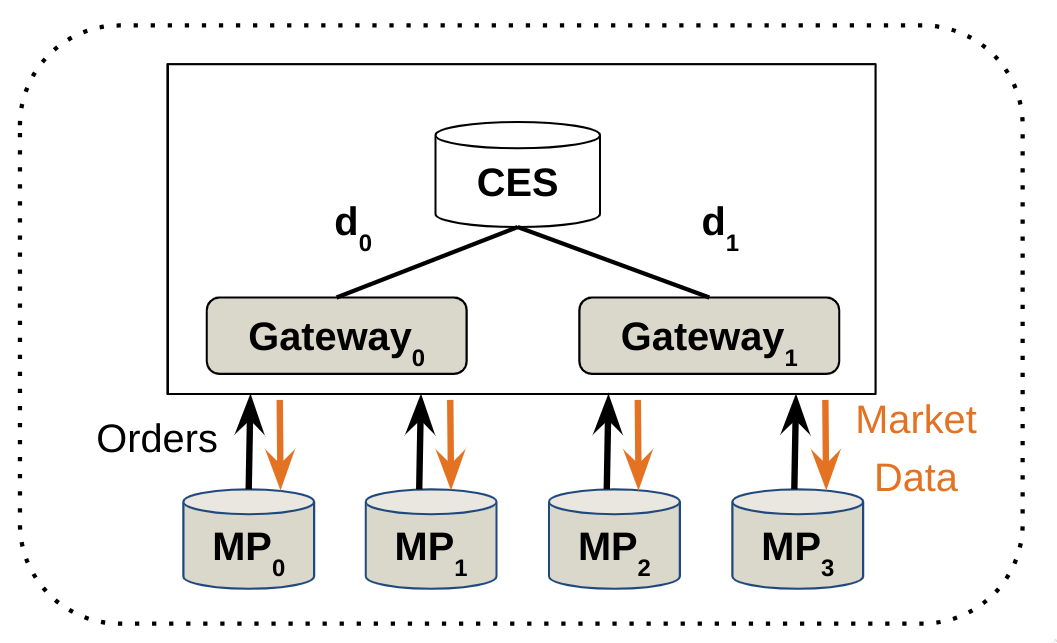
\includegraphics[width=0.4\textwidth]{./assets/architecture.png}
%     \caption{An Exchange's Infrastructure}
%     \label{fig:exchange}
%   \end{center}
% \end{figure}

\textbf{\textit{Gateways}}. The gateways are structures placed between traders
    and the CES. Their responsabilities consist of routing orders and market data, as 
    well as protecting the CES from abuse, e.g., unauthenticated or invalid orders. Within
    the on-premise clusters gateways are made to be equidistant to the CES as to 
    ensure fairness regarding communication delays between the gateways and the 
    central exchange.

\begin{figure}[h!]
  \begin{center}
    \begin{minipage}{0.45\textwidth}
      \centering
      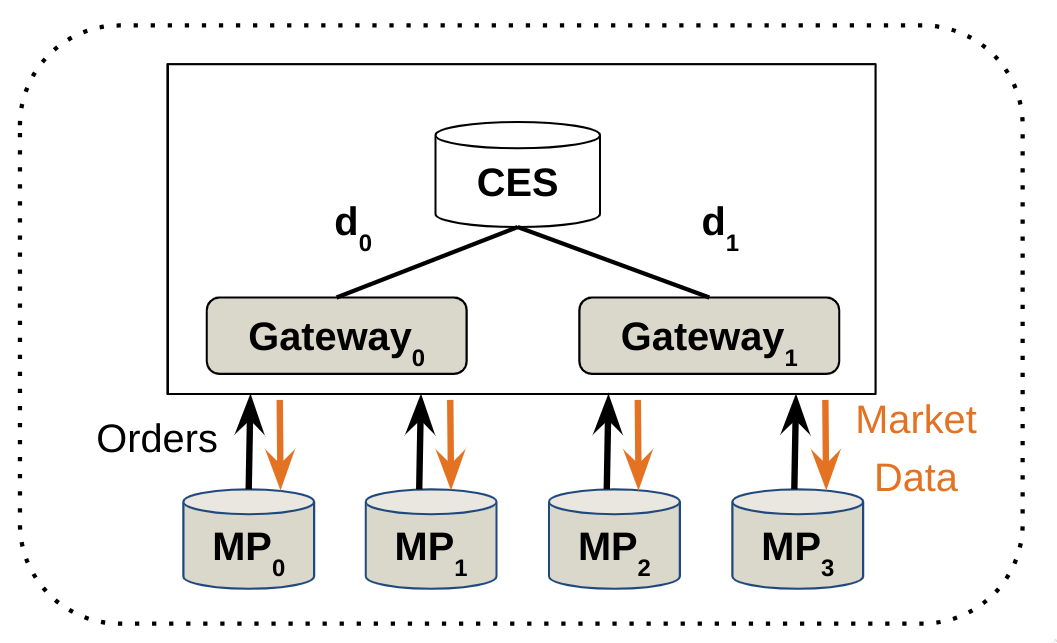
\includegraphics[height=0.20\textheight]{./assets/architecture.png}
      \caption{On-premise Infrastructure}
      \label{fig:exchange}
    \end{minipage}
    \hfill
    \begin{minipage}{0.45\textwidth}
      \centering
      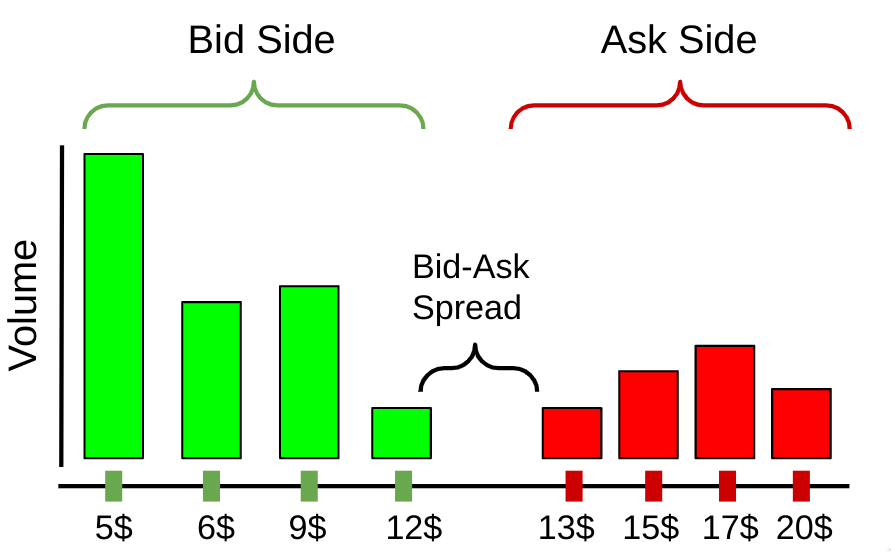
\includegraphics[height=0.20\textheight]{./assets/LOB.png}
      \caption{Limit Order Book}
      \label{fig:lob}
    \end{minipage}
  \end{center}
\end{figure}

\section{Migrating Financial Exchanges to the Cloud}
Given the demanding network performance of financial exchanges, the use of 
on-premise data centers is the prevailing standard.
However, the cloud displays well-known advantages as a medium for communication. 
These include flexibility, scalability, robustness and potential cost savings. 
On the other hand, the public cloud also exhibits high latency variance \cite{cloudy}.
Additionally, it does not provide low-level engineering control to cloud-tenants such as switch-based multicast. 
As a result, cloud-based systems implement multicasting by directly unicasting a copy of a message 
to each recipient \cite{nezha, cloudex, octopus, dbo}.


A fundamental characteristic of a financial exchange is the ability to disseminate data
    to market participants in a fair manner. 
That is, all MPs receive updates to the market almost simultaneously, as to not allow 
    unwanted arbitrage opportunities.
Without native solutions to enable multicasting and the significant serial 
    delay of direct unicasting, a clear problem is presented 
    to achieve the possible migration of financial exchanges to the public cloud.

\section{State of the Art}
\subsection{Jasper: Fair Multicast for Fin. Exchanges on the Cloud}
A siginificant project in this domain is Jasper \cite{jasper}, which offers 
a modern implementation of a financial exchange on the public cloud. 
This work realizes a multicast service that achieves low latency of less than 
250 µs and a latency difference of less than 1 µs across 1,000 multicast receivers.
To accomplish this, a series of techniques are employed.


\textbf{\textit{Overlay Proxy Tree}}. This is the starting point for Jasper's design 
    and borrow's the concept of trees to scale communication to a larger number of 
    receivers, while improving latency in comparison to direct unicasting \cite{matsuoka, twotree}.
    The structure of the tree with Depth (\textbf{D}) and fan-out (\textbf{F}) has been empirically established 
    as seen in Equations [\ref{eq:fanout}, \ref{eq:depth}].
    % Ideally, F has been fixed to 10, while the value of D is derived via [$log_{10}{(N)}$], where N is the number 
    % of receivers.

\begin{align}
F &= 10 \label{eq:fanout} \\
D &= \log_{10}{(N)} \label{eq:depth}
\end{align}

\textbf{\textit{Clock Synchronization}}. \cite{hyugens}


\chapter{Implementation/Results}
\section{Implementation}
Details regarding implementation and/or simulation are given in this chapter. The considered setup and the parameters used are introduced and discussed. Also, the general evaluation methods can be presented. (Note: Code should not be part of this chapter. If it makes sense to introduce it into the thesis, it should be placed in the appendix.)

\section{Results}
Results of the performed investigations are presented here. Interpretations for the observed effects are given and the impact of investigations is discussed. 

%  Conclusions (Zusammenfassung):
\chapter{Conclusions and Outlook}

The thesis is concluded here. The considered problem is repeated. The contribution of this work is highlighted and the results are recapitulated. Remaining questions are stated and ideas for future work are expressed. 
%\chapter{Formatting}

\section{Figures and Tables}
Figures and tables need to include a caption. This can be done with the LaTeX-command \texttt{\bslash caption$\lbrace\rbrace$}. To be able to reference figures and tables, a \texttt{\bslash label$\lbrace\rbrace$} must follow the caption.

\begin{figure}[h!]
  \begin{center}
    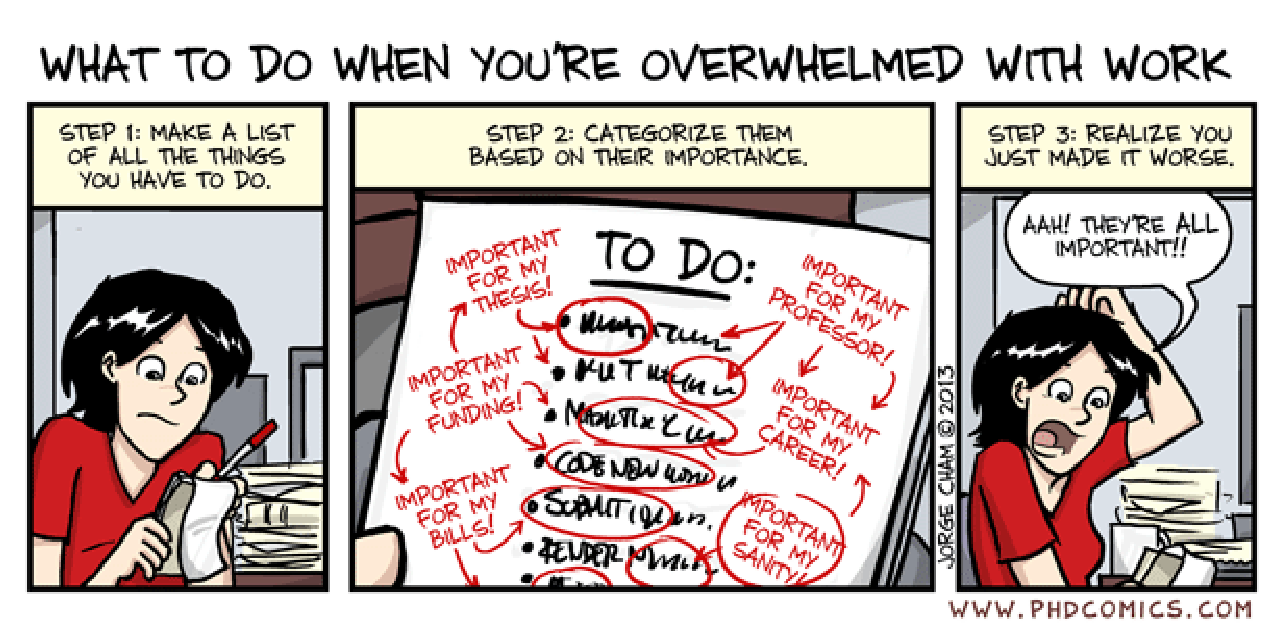
\includegraphics[width=0.6\textwidth]{phd112013s.eps}
    \caption{Ein PHD Comic}
    \label{fig:ToUseWithReference}
  \end{center}
\end{figure}

\begin{table}[b]
\begin{center}
\begin{tabular}{|l |c|}
\hline 
\textbf{Parameter} & \textbf{Value} \\
\hline  
\hline 
Transmission Power & 23~dBm\\
\hline 
Center Frequency & 2.6~GHz\\
\hline 
Channel Bandwidth & 15~kHz\\
\hline 
Shadowing Correlation Distance & 40~m\\
\hline 
Noise Density & -174~dBm/Hz\\
\hline 
Antenna Heights & 1.5~m\\
\hline 
\end{tabular}
\caption{Simulation Parameters and Values}\label{tab:param_table}
\end{center}
\end{table}

The labelled figures and tables can be referenced via \texttt{\bslash ref}, e.g. ~Figure~\ref{fig:ToUseWithReference}.
\newpage

\section{Referencing}
Literature references are included e.g. like this:\\
``..., as shown in \cite{eberspaecher97},, ...'' or ``... there are several approaches \cite{arnaud99,griswold90} ...''

% Appendix (Anhänge), could have multiple chaper-files:
\appendix
\chapter{}
The appendix may contain some listings of source code that has been used for simulations, extensive proofs or any other things that are strongly related to the thesis but not of immediate interest to the reader. 

% Abbreviations (Abkürzungsverzeichnis):
\chapter{Abbreviations}
\begin{table}[h]
\begin{tabular}{ll}
CES & Central Exchange Server \label{abbr:CES}\\
MP & Market Participant \label{abbr:MP}\\
\end{tabular}
\end{table}




% References (Literaturverzeichnis):
% a) Style (with numbers: use unsrt):
\bibliographystyle{alpha}
% b) The File:
\bibliography{Bibliography}


%%%%%%%%%%%%%%%%%%%%%%%%%%%%%%%%%%%%%%%%%%%%%%%%%%%%%%%%%%%%


%%%%%%%%%%%%%%%%%%%%%%%%%%%%%%%%%%%%%%%%%%%%%%%%%%%%%%%%%%%%


%%%%%%%%%%%%%%%%%%%%%%%%%%%%%%%%%%%%%%%%%%%%%%%%%%%%%%%%%%%%
\end{document}
